\chapter{可信机器学习基础}
\label{chap:trust-foundations}

上一部分“机器学习理论”回答的是一个统计问题：在给定假设空间、学习目标和抽样关系后，怎样用有限样本推断模型在\emph{同一个总体}上的期望风险，泛化界给出了这种推断的误差和失败概率。但学会预测只是第一步。一个模型真正被放进系统、替人做决定时，我们还要回答另一组问题：它的输出会触发什么行动？行动出错的后果由谁承担？环境变化后原来的测试结论还作数吗？泛化界只说明预测误差在原总体上有多大，不涉及行动、承担者和时间变化，因此这些问题不能只靠“测试集风险低”来回答。

先看一个贯穿全章的对比。同一个垃圾邮件预测结果，系统可以只是把可疑邮件放进一个\emph{可以恢复}的隔离文件夹，也可以\emph{直接永久删除}。两种用法使用的是同一个模型、同一个预测，但后果完全不同：隔离误判了还能找回，永久删除则可能让收件人错过一封求职通知或丢失一份合同附件。不仅如此，决定如何使用系统的人（开发或采购方）和承担误判后果的人（收件人）往往不是同一个。因此，从“模型会不会预测错”进入“能不能这样使用模型”时，要分清几件不同的事：被约束的究竟是预测误差、输出概率是否可靠、预测区间是否覆盖真值，还是“模型+处置规则”共同造成的行动损失；用户有没有质疑和复核的渠道；条件改变后由谁监测、出错后如何补救。这些都不是泛化误差自动包含的信息。

举个最简单的数字：一个邮件分类器在测试样本上达到了97\%的准确率。这个数字本身完全无法回答“能不能让它自动删除邮件”。它没有区分错误的类型（误拦正常邮件 vs. 漏放垃圾邮件），没有说明这两类错误的代价，也没有说明测试样本是否代表未来的邮件、收件人是否有机会发现和纠正误判。准确率给的是\emph{预测质量}的一个侧面，而“授予多大权限”是一个\emph{使用决策}，需要的信息多得多。

\term{可信机器学习}（trustworthy machine learning）研究的正是这一使用问题：模型及其使用过程需要满足哪些\emph{明确的要求}，又需要哪些\emph{证据}才能证明这些要求得到了满足。白话地说，它要回答“凭什么可以把这项工作交给模型、交到什么程度”。“可信”不是一个可以用单一分数概括的总评价，而是一组需要分别检验的主张：一个模型输出的概率可能很可靠，却会泄露训练数据中的个人信息；它可能抵御了某类对抗攻击，却对某个少数群体频繁出错。一项主张成立不能推出另一项成立，有些性质之间甚至互相冲突。因此不能用一个“综合可信分”让各项互相补偿：隐私泄露不能因为准确率高就被抵消，第~\ref{sec:trust-requirements}节会把这一点写成约束而不是加分项。

还要先界定本部分能做什么、不能做什么。我们讨论的是\emph{技术可信性}：用模型、数据、算法和技术系统本身能够提供的证据，说明哪些主张成立、成立到什么程度。这些证据可以提交给组织审批、法律合规审查和公共治理讨论使用。但是否部署、授予多大权限、出了事由谁负责、剩余风险由谁接受，这些是\emph{有权主体}（依法依章承担责任的人或机构）结合领域规则、受影响者的陈述和补救需求作出的\emph{治理决定}；技术测试本身既不能代替授权，也不能代替法律判断。把这条边界讲在前面，是为了避免“测试通过=可以合法/应该部署”的误读。

本章给出后面各章共用的分析框架，它沿着三个依次递进的问题展开。第一，把使用情境翻译成\emph{明确的要求}：不是笼统地说“要可靠”，而是写清约束哪个可测量的量、对谁、在什么范围内、阈值是多少。第二，评估\emph{证据}的强度：哪些理论结论、抽样测试、压力测试或机制分析能够支持这条要求，反例和未覆盖的情形是什么。第三，安排\emph{失效后的处置}：什么条件变化会让结论失效、由谁监测、触发后如何限制使用和恢复。第三个问题之所以单列，是因为前两步得到的结论都绑定在测试时的数据、模型和权限上，系统一旦变化，结论就可能过期。这三个问题（要求、证据、生命周期）将贯穿可靠性、鲁棒性、公平性、目标对齐、可解释性、隐私和对抗安全各章；本章用一个邮件隔离的完整例子把它们串起来，最后按七项性质梳理研究内容和研究历史。

图~\ref{fig:trust-technical-scope}把技术证据与法律合规、组织审批、公共治理放在同一张使用情境图中。需要强调的是，图中的交叉区域只表示各方会讨论一些共同议题，\emph{不表示}一种判断能推出另一种：技术检验通过，既不等于部署合法，也不等于已经获得批准或得到公众认可；反过来，法律或管理要求也需要相应的技术证据才能落地。阅读本章和后面各章时，请始终把“技术上能证明什么”和“谁有权据此作什么决定”分开。

\begin{figure*}[htbp]
  \centering
  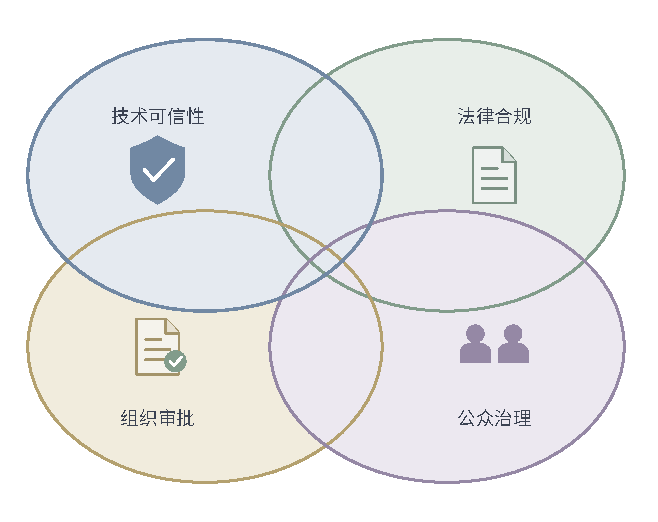
\includegraphics[width=111.404mm]{figures/06-foundations/03-trustworthiness/tikz/trust-technical-scope/figure.pdf}
  \caption{蓝色轮廓标出本书讨论的技术证据，其他区域表示法律合规、组织审批与公共治理。交叉处只示意共享议题；边界及面积不表示集合度量、逻辑包含或责任继承，各主体仍依自身要求判断。}
  \label{fig:trust-technical-scope}
\end{figure*}

\section{技术可信性的范围与三个层次}
\label{sec:trust-context}

在进入三个层次之前，先固定一条分析主线，即“预测—处置—后果”。模型给出的只是一个预测（例如“这封邮件是垃圾邮件的概率为0.9”），系统再按某条规则把预测变成一个\emph{处置}（放行、隔离、删除或转人工），处置作用在真实世界后才产生\emph{后果}（错过通知、泄露诈骗等）。风险必须沿这条链条一直算到后果，而不能停在预测处。算清后果还要回答两个范围问题：一是损失\emph{落在谁身上}，这决定损失怎样计量；二是结论\emph{适用于哪些人、哪些输入和环境}，这限定结论能推广到哪里。一个脱离了这两条信息的性能数字，无法决定系统应被授予多大权限。有了这条主线，我们可以按“提出什么要求—用什么证据支持—证据何时失效”分三层组织分析。

第一层把“系统属性”写成可判定的“规范要求”。“可靠”“隐私”“公平”这些词只是\emph{系统属性}的名称，它们告诉我们要考察哪一类性质，本身却无法被测试，因为没有说明测什么、测到多少算合格。规范要求则是能够判定成立与否的具体陈述。要让一条要求可检验，必须补充四件事：约束的对象是谁（全体用户还是某个人群）、评价单位是什么（单封邮件、单个用户一周的使用，还是一次完整流程）、适用范围是什么（哪些语言、哪些输入）、以及允许发生什么事件、阈值或程序条件是什么。例如，“邮件隔离要可靠”应写成“自动隔离的邮件中，正常邮件所占比例不超过2\%”；“数据使用要合规”应写成一条可检查的授权流程（谁、在什么审批下、能访问哪些字段）。

第二层检查证据是否真的支持这条要求。提出要求后，要判断手头的证据能支持到什么强度。理论结论（如泛化界、覆盖率定理）必须连同它的假设和量词一起读。这里的量词指结论“对什么成立”：是对所有输入都成立，还是对随机抽样取平均后成立。有的定理约束的是“重复抽样的平均”，并不保证“每个固定输入”，误用量词就会夸大结论。抽样检验必须交代数据是怎样取得的：随机样本可以估计总体风险，刻意构造的困难样本只能用于找缺陷而不能估计部署失败率。压力测试、对模型内部机制的分析、以及对使用者的人因评价，则各自补充其他手段看不到的失效模式。还要把反例和剩余不确定性与有利结果\emph{一起}记录，否则无法判断结论到底有多强。

第三层规定结论在运行中何时失效、如何处置，我们称之为生命周期条件。任何证据都对应一组条件，条件变了结论就可能失效。这一层要事先写清：哪些变化（数据来源、模型版本、权限、使用方式）会使旧结论暂停适用；由谁负责持续监测；一旦触发，怎样限制使用（降级、停用、转人工）、如何回退到已验证版本、怎样补救并恢复到可以重新评价的状态。技术材料提供作出这些判断所需的依据，而是否接受剩余风险、是否批准继续部署，仍由有权主体决定。

三个层次各有不可替代的职责，跳过任何一层都会得到站不住的结论：没有明确要求，测试就不知道在支持什么行动；没有证据，要求只是愿望；没有生命周期安排，数据、模型、权限或用法已经改变，系统却仍在沿用几个月前那份测试报告的结论。下面先从最具体的一环开始：邮件处置的后果怎样量化。

图~\ref{fig:trust-three-layers}在三个层次上同时标出三类角色：提出要求的任务方、准备并独立复核证据的技术方、以及作出风险决定并执行处置的有权主体和运行方。要强调的是，这些职责必须落实到\emph{真实的授权记录}里（谁有权批准、谁有权停用），而不能只停留在示意图上。算法可以高速给出计算结果，却既不能替人承担责任，也不能自行决定这套分工。

\begin{figure*}[htbp]
  \centering
  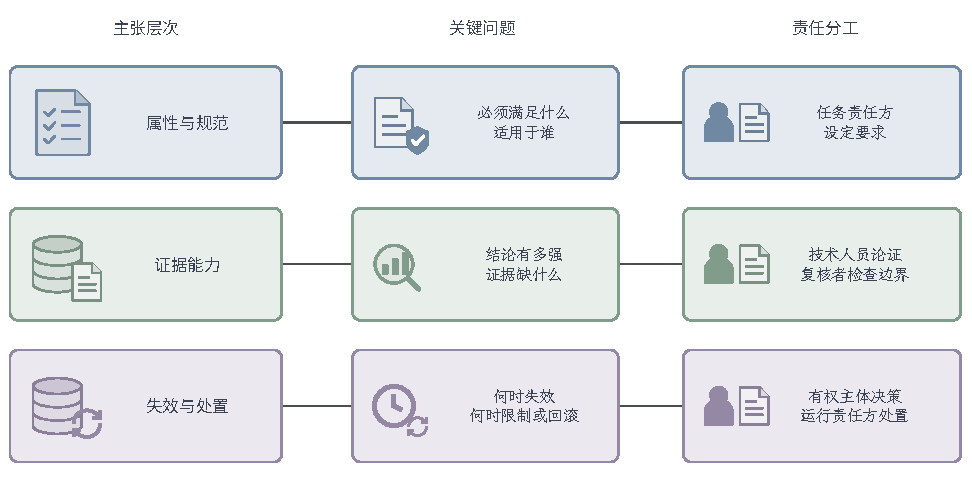
\includegraphics[width=164.600mm]{figures/06-foundations/03-trustworthiness/tikz/trust-three-layers/figure.pdf}
  \caption{要求、证据及失效处置构成可信主张的三个层次。系统属性选择考察维度，规范要求确定条件；证据限定结论强度；生命周期条件确定暂停沿用和响应。三行分别连接任务方的要求、技术论证与独立复核、有权主体的风险决定和运行方处置。横线只表示同层对应，教学分工仍需由真实授权与审批落实。}
  \label{fig:trust-three-layers}
\end{figure*}

\subsection{从预测结果到实际后果}

要比较“隔离”和“删除”这两种用法，先得把“预测如何变成行动”写成可以计算的形式。这里要分开三样东西：邮件本身、模型看到的内容、以及决定行动的规则。用$o$表示一封邮件的原始记录（正文、发件人、附件等），用$r$表示把记录转换为预测输入的规则（例如只抽取正文的词频），记$\bm x=r(o)$。模型实际读取$\bm x$并给出$f(\bm x)$，例如垃圾邮件概率。系统再通过\emph{决策规则}$d$，把模型预测与本次任务允许读取的原始字段共同转换为行动：
\[
 a=d(f(r(o)),o).
\]
例如概率低于0.2放行、高于0.98隔离、中间转人工，也可在权限允许时检查发件域名。域名若未进入$r(o)$，就不是预测器$f$可见的特征；决策规则能够读取它，并不表示模型已用它预测。这个拆分说明，保持表示规则$r$和模型$f$不变、只改变$d$，系统后果仍可能改变，这正是“同一模型、不同权限”的数学表达。

为了用\emph{同一把尺子}比较处置，先引入行动损失：记邮件的真实状态为$y$（是否真为垃圾邮件），用$L(a,y)$表示采取行动$a$后按当前成本约定计量的损失。这里先采用固定教学成本，即同一行动和真实状态使用相同成本值。它不同于零一损失，可以区分误拦正常邮件和漏放垃圾邮件的代价。令\emph{部署分布}$\mathcal P$为进入评价范围的原始记录与标签$(o,y)$的联合分布，整个“表示、模型与决策规则”系统的期望损失为
\begin{equation}
 R_{\mathrm{sys}}(f,r,d)
 =\mathbb E_{(o,y)\sim\mathcal P}
 L\bigl(d(f(r(o)),o),y\bigr).
 \label{eq:trust-system-risk}
\end{equation}
式中期望对部署分布中的邮件取平均，被平均的是“这封邮件经过表示、预测和决策后采取的行动，在其真实状态下造成的损失”。本章比较处置时固定$r$，下文简写为$R_{\mathrm{sys}}(f,d)$。在这个约定下，风险同时取决于模型$f$、规则$d$和部署分布$\mathcal P$，任一项改变都可能改变损失。反过来不成立：两套系统的风险数值相同，并不说明它们的组成相同，例如规则只在概率为零的记录上有差别时，期望值不变。

这个式子与理论部分的期望风险形式相同，区别在于被计分的对象。分类器的零一损失只问预测对不对，衡量\emph{预测质量}；这里的行动损失问行动造成多大代价，衡量\emph{使用代价}。正确率较低的模型可能因少犯昂贵错误而使系统损失较小，下面的例子直接演示这一点，因此两者不能互相替代。

图~\ref{fig:trust-decision-consequences}保持模型预测$p=f(\bm{x})$不变，分别画出“隔离”和“永久删除”两条行动链：两条链的起点是同一个分类结果，但一条保留了原件、可以找回，另一条销毁了原件；链条末端收件人承担的后果（能否找回、是否错过期限）完全不同。比较系统时要看的是\emph{链条末端}的后果，而不是链条起点处的预测是否正确。

\begin{figure*}[!htb]
  \centering
  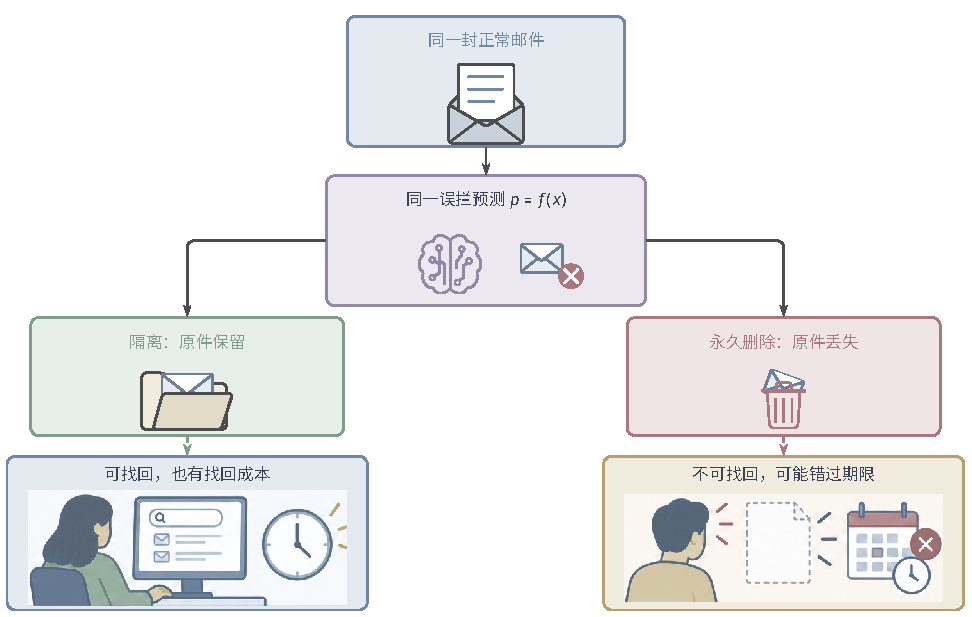
\includegraphics[width=164.600mm]{figures/06-foundations/03-trustworthiness/tikz/decision-consequences/figure.pdf}
  \caption{保持$p=f(\bm x)$不变，比较同一正常邮件误拦后的隔离与永久删除。左侧保留原件可供找回，右侧删除原件；末端收件人可能承担找回成本或错过期限。完整流程损失还需考虑邮件价值、发现延误和恢复成本；图中示意需要纳入的后果，不表示两变量教学成本$L(a,y)$已经表达所有差异。情景为构造，保留原件并不保证及时找回。}
  \label{fig:trust-decision-consequences}
\end{figure*}

\begin{example}[准确率与行动损失]
\label{ex:trust-mail-cost}
在一个构造的1000封邮件测试样本中，模型甲误拦10封正常邮件、漏放20封垃圾邮件，模型乙误拦2封正常邮件、漏放40封垃圾邮件。按正确封数计算，甲的准确率为97\%，乙为95.8\%。现在把每次误拦损失设为10、每次漏放损失设为1：甲产生的总损失为$10\times10+20=120$，乙为$2\times10+40=60$。同一测试样本上，乙虽然正确率较低，却减少了在此损失设定下更昂贵的错误，因此总行动损失较低。比较结论仍限于这批样本和成本设定，不能单独决定使用权限。
\end{example}

这个例子虽然用的是人为指定的代价，但它清楚地说明一件重要的事：\emph{按正确率给模型排序，和按行动损失给系统排序，结果可能相反}。这种排序同时取决于模型产生的错误构成和每类错误的代价：固定错误计数而改变成本比，或固定成本而改变误拦与漏放数，都可能改变排序。真实邮件流程还涉及每封邮件的价值、处理延误、申诉人力及恢复时间。若这些因素会改变比较，就要给损失增加相应记录或轨迹变量，或明确固定成本是在什么条件下对后果取过平均，不能只由$(a,y)$读出全部差异。例如，隔离若能及时找回，代价可能远小于永久删除；但如果用户一直没发现被误拦，即使原件还在，也错过了合同期限，保留原件并没有真正实现补救。因此评价不能只看模型输出那一刻，而要追踪从预测到处置再到补救的\emph{完整流程}。

既然不同错误有不同成本，就可以反过来\emph{从成本推导决策阈值}，而不是凭习惯取0.5。仍只比较“隔离”和“放行”两个动作，在看到当前邮件的条件下选期望损失更小的那个。设$p$是这封邮件为垃圾邮件的真实条件概率；误拦一封正常邮件的成本为$c_{\mathrm{fp}}>0$，漏放一封垃圾邮件的成本为$c_{\mathrm{fn}}>0$，处理正确时不计成本。隔离只在邮件其实正常（概率$1-p$）时才造成损失，期望损失为$(1-p)c_{\mathrm{fp}}$；放行只在邮件真是垃圾（概率$p$）时造成损失，期望损失为$pc_{\mathrm{fn}}$。当隔离的期望损失更低时就应隔离。不等式$(1-p)c_{\mathrm{fp}}<pc_{\mathrm{fn}}$两边加上$pc_{\mathrm{fp}}$得$c_{\mathrm{fp}}<p(c_{\mathrm{fp}}+c_{\mathrm{fn}})$，再除以正数$c_{\mathrm{fp}}+c_{\mathrm{fn}}$，得到阈值规则
\begin{equation}
 p>\frac{c_{\mathrm{fp}}}{c_{\mathrm{fp}}+c_{\mathrm{fn}}}.
 \label{eq:trust-cost-threshold}
\end{equation}
在阈值处两种动作的期望损失恰好相等，选哪个都一样。这条规则说明：误拦的代价相对越高，就越要求模型有把握才允许隔离。例如$c_{\mathrm{fp}}=10,c_{\mathrm{fn}}=1$时阈值为$10/11\approx0.91$；只有当两类错误代价相等时阈值才是0.5。所以0.5只是等代价下的特例（可参考\BookChapterRef{chap:decision-theory-and-dynamic-risk}{卷2《数学准备：概率、因果与决策》第6章“策略的价值与优化”}）。

推导中用的是\emph{真实}条件概率$p$，实践中代入的却是模型\emph{估计}出的概率，因此整条决策规则的质量取决于概率估计本身是否可靠。这里要避免一种过度解读：如果我们把邮件按预测概率分箱（如0.1一档），发现“预测为0.3的那一档邮件中真有约30\%是垃圾邮件”，这只是\emph{分组平均}意义上的校准证据，并不能证明模型对每一封具体邮件给出的0.3都是准确概率。概率校准、区间覆盖以及相应的检验方法，将在第~\ref{chap:trust-reliability}章展开。

\begin{example}[增加复核选项后的决策]
\label{ex:trust-review-cost}
沿用教学成本$c_{\mathrm{fp}}=10$、$c_{\mathrm{fn}}=1$，再加入一个固定成本为0.2且能够无误确认标签的人工复核选项。隔离、放行和复核的候选损失分别为$10(1-p)$、$p$和0.2。比较三者：放行优于复核要求$p<0.2$；隔离优于复核要求$10(1-p)<0.2$，即$p>0.98$；而$p<0.2$时$10(1-p)>8$，隔离不会更优。于是$p<0.2$时放行损失最小，$p>0.98$时隔离损失最小，中间的$0.2<p<0.98$则由复核占优；两个端点各有两种行动成本相等。复核区域来自成本比较，不需要模型额外预测一个“犹豫”类别。
\end{example}

这个例子之所以能用一个固定的0.2代表复核，是因为假设了人工\emph{一定能判断正确}。现实中要放松两点：若复核员也会误判，就要把误判概率和后果计入；若复核队列很长、用户需要等待，等待成本也应进入第三项。此时复核的损失不再是常数，中间区间的宽度会随之变化。

还要把视野放大：判断“该不该上这个模型”，不能只在两个模型之间比准确率，而应在\emph{相同条件}下把它与“完全人工处理”“用一条简单规则”“只授予较低权限的自动化”等替代方案一起比较期望损失。两个模型的准确率对比完全没有涵盖这些流程级替代方案。

现实中误拦和漏放的成本往往无法精确给出，只能给出一个大致区间（例如“误拦一封重要邮件的代价至少是漏放的5倍、至多20倍”）。这时的做法是\emph{成本敏感性分析}：让成本比在这个区间内逐档变化，对每一档重新计算各可行方案的期望损失并比较。成本区间应由领域约束和有权主体\emph{在看到结果之前}声明，而不能事后挑一个让某方案获胜的值。解读方式很直接：如果一个方案只在成本比很窄的范围内占优，说明结论强烈依赖精确的成本判断、较脆弱；如果它在整个声明区间内都比替代方案损失低，结论对成本估计的不确定性就不敏感。还要区分两种“改变条件”：这里改变的是\emph{使用假设}（错误代价），而第~\ref{chap:trust-robustness}章讨论的是输入分布或环境本身发生改变，两者不能混为一谈。

式~\eqref{eq:trust-system-risk}隐含了一个常被忽略的假设：真实标签$y$是\emph{固定的、不随我们采取的行动而改变}的。对邮件分类这通常合理——一封邮件是不是垃圾邮件，不会因为我们隔离或放行它而改变。但在资源分配类任务中，行动本身会\emph{改变}标签。例如用一个分数决定谁能参加培训，而培训会提高后续成绩：这时“参加培训者后来成绩好”可能部分是培训的效果，不全是分数选得准。把历史上“高分者参加培训后的成绩”直接拿来，无法回答“如果把名额给低分者会怎样”，因为低分者\emph{没有}被培训过、根本观察不到他们在培训下的结果。要比较这类行动，必须显式描述每个候选行动\emph{会导致}的结果分布，并通过额外的随机化实验或因果假设来估计；历史行动下观察到的$y$不能直接当作所有行动共用的固定标签。这一“预测问题 vs. 干预问题”的区分，在第~\ref{chap:trust-fairness}章讨论长期分配后果时还会再次用到。

\subsection{风险的承担者与使用范围}

行动损失确定之后，紧接着要回答“这笔损失由谁承担”。在很多系统里，\emph{使用系统的人}和\emph{承担后果的人}并不是同一方：招聘筛选模型为用人方节省了筛简历的工作量，但被错误拒绝的求职者承担了失去机会的后果；信贷模型提高了放款方的效率，被错误拒贷的申请人承担损失。因此一份完整的评价不能只记录系统给运营方带来的收益，还要同时记录：错误负担落在哪一方、受影响者有没有机会发现错误、有没有申诉和纠正的渠道。开发者在日志里最容易测量的指标（吞吐量、点击量、整体准确率）往往恰好覆盖不到这些由他人承担的影响。

还要注意，同一种错误的代价和发生概率会随使用条件变化：不同语言、不同设备、不同时间段、不同输入质量（模糊、缺字段）和不同用户群体，都可能有不同的风险。因此部署范围里的每一句“适用于某类输入”都应对应一个\emph{可以检查的条件}（例如“正文为中英文文本、字符编码正常”），使系统在运行时能判断当前输入是否在范围内；对范围外的输入，则要事先安排识别手段、限制使用（不自动决策）或转交人工。至于环境变化具体会怎样破坏训练时学到的规律，是第~\ref{chap:trust-robustness}章的主题。

一旦把“会怎样失效”放进具体使用情境，还会发现许多\emph{与预测对错无关}的危害：一个答案可能内容正确，却在生成过程中泄露了训练数据里的个人信息；模型可能准确完成了指令，却越过了被授予的权限（删除了不该删的文件）；也可能被外部内容（如网页或邮件中的文字）诱导，偏离用户真正的任务。这些失效路径分别对应后面的隐私、目标对齐与对抗安全章节。先把路径明确出来，才能选择对应的保护措施，而不是用一个笼统的“准确率高”掩盖它们。NIST的人工智能风险管理框架也主张从使用情境出发来识别、测量和管理风险；但套用这类框架的原则时，仍需把每一条落实到当前系统的具体对象和阈值上，原则本身不能代替论证\scite{nist2023rmf}。

\section{系统属性与规范要求}
\label{sec:trust-requirements}

第~\ref{sec:trust-context}节已经列出系统会造成哪些危害、由谁承担。本节要把这些危害转化为\emph{可以判定成立与否的要求}。这件事包含三个相互衔接的工作：把要求写成能观察、能测量的主张（例如“误拦比例不超过2\%”），而不是停留在“要安全”；检查要求清单是否遗漏了重要情境（某些子类型、某些人群）；处理多条要求之间的关系，它们可能互相支持，也可能直接冲突。之所以一定要落到可观察事件，是因为“用户受损”只是笼统描述，没有给出所测事件或尺度，无法据以判断一次修改是好是坏。金额、延误时间和误删件数有时可以直接记录，但仍须说明属于哪类后果、落在谁身上、怎样对应行动规则，才能判断修改是否减少了所关心的损失。反过来，如果只优化一个与行动无关的数值（例如一个没有明确用途的“置信度”），数值变好了也可能与使用目的毫无关系。

\subsection{可信性要求的具体表达}

以邮件任务说明一条规范要求应包含的要素。“系统要可靠”至少可以落实成两条很不同的要求：一是“被自动隔离的邮件中，正常邮件所占比例不超过2\%”；二是“对某一人群给出的预测区间，真值落入区间的比例不低于90\%”。这两条约束的\emph{承载对象}不同（一个是隔离动作的后果，一个是概率/区间输出），分母也不同。因此每一条都必须单独声明四件事：评价单位（以什么为一次观测）、总体范围（在哪些邮件、哪段时间上）、错误事件（发生什么算失败）、容许水平（阈值多少）。只有写清这些，才能判断一份测试报告\emph{究竟支持了哪一条主张}——一个95\%的总体准确率既不能推出隔离精确率，也不能推出区间覆盖率。

评价单位的选择还会\emph{数值地}改变风险，不能混用。以“单次调用”为单位测得的失败率，不能直接当作“一个用户连续使用一周”的失败率：如果每次调用独立、单次失败概率为$q$，那么$m$次全部成功的概率是$m$个$1-q$相乘，即$(1-q)^m$，一周调用$m$次中\emph{至少失败一次}的概率为$1-(1-q)^m$。取教学数值$q=0.1\%$、$m=200$，这个概率约为18\%：单次看来很小的失败率，对一周的使用者已不再小。因此多步骤、长周期的任务要分别评价两类性质：每一步是否可靠，以及整条流程最终是否达成目标——单步都达标，并不自动保证长链条的结果达标。

明确评价单位后，还要选择\emph{用什么数学形式}表达要求，不同形式适合约束不同性质。对于可以用钱或时间补偿的代价，用\emph{平均行动损失}来比较方案最合适；但另一些性质不适合被平均掉，例如“发生灾难性错误的概率”“某个人群必须达到的下限”“只有授权角色才能访问某类数据”，这些更适合写成\emph{单独的约束}（硬性上限或必须满足的程序条件），而不是放进一个可被其他收益抵消的平均值。设任务、可供选择的模型、允许的行动和权限边界共同确定了候选模型族$\mathcal F$和决策规则集合$\mathcal D$。在要求都可量化时，选择系统就可以写成一个带约束的优化问题：在满足全部硬约束的方案中，选平均行动损失最小的模型与规则，
\begin{equation}
 \begin{aligned}
  \min_{\substack{f\in\mathcal F\\d\in\mathcal D}}\quad
  &R_{\mathrm{sys}}(f,d)\\
  \text{s.t.}\quad
  &G_j(f,d)\leq b_j,\quad j=1,\ldots,m.
 \end{aligned}
 \label{eq:trust-constrained-objective}
\end{equation}
其中$G_j(f,d)$是第$j$项要求的测量量（例如隔离邮件中的正常邮件比例），$b_j$是它的容许上限，$m$是要求条数。这个写法体现了一个重要的决策次序：\emph{先用约束排除所有不可接受的方案，再在剩下的方案中按平均损失挑最好的}。也就是说，无论一个方案平均损失多低，只要违反了某条硬约束（如隐私、公平下限、权限），它一开始就不在候选集中，不能靠其他方面的高收益“赎买”过关。使用这个优化式还要注意两个技术细节：它要求可行集非空且最优解能取到，否则应如实报告“约束之间互相矛盾、无可行方案”；若可行方案的损失只能无限逼近某个值而取不到，则报告这个下确界（最大下界），并说明实际采用的方案离它多远；对于那些无法合理量化的程序性要求（如“必须经过人工审批”），应保留在公式之外作为流程约束，而不能硬造一个分数假装它已被涵盖。

\subsection{可信性要求的完整性}

一个常被忽视的现象是：即使所有模型都满足了现有的风险要求，它们在真正关心的部署行为上仍可能差别很大。\term{欠规定性}（underspecification）指的就是这种\emph{信息缺口}——给定的训练任务和评价条件，足以让一大批模型都“达标”，却不足以区分它们在新环境、子群体或压力情境下的不同表现。典型的产生方式是：多个不同的预测函数可以利用在训练分布上等价的规律，因而在现有训练与测试中无法区分，而随机初始化、样本顺序等可能使训练过程选中不同函数；一旦部署环境使这些规律不再等价，不同训练轮次得到的模型就会表现迥异。D'Amour等人在医学影像、自然语言等多条流水线中都观察到这一现象。它提醒我们：除了检查“某个模型是否过拟合”，还要检查“训练和评价条件本身能不能把行为正确的模型筛选出来”\scite{damour2020underspecification}。

用一个构造的邮件例子把“过拟合”和“欠规定性”区分开。假设在历史数据中，内容特征$x_1$（邮件正文是否含某类措辞）和页脚特征$x_2$（页脚是否带某个推广标识）\emph{始终同时出现}，而标签恰好由它们共同决定。于是，一个只用$x_1$的分类器和一个只用$x_2$的分类器，在任何同分布测试集上都得到100\%正确——它们看起来一样好。问题在于，增加再多\emph{同一来源}的测试邮件，也只能更精确地确认“$x_1$与$x_2$总是一起出现”，无法判断部署后哪条规律仍成立。假如新月份中推广标识消失、但正文措辞与垃圾邮件的关系保持，那么只用$x_2$的模型会失效而只用$x_1$的不会；可这一差异在旧分布下根本测不出来。此时缺的不是更多同分布数据，而是一个\emph{能把两条规律区分开的新情境}。

补上这个缺口需要额外信息，它可以用在训练端，也可以用在评价端。训练端的做法是让训练过程本身偏向正确规律：收集$x_1$与$x_2$不再同现的其他环境的数据，用结构约束限制模型只读取正文，或写入“页脚标识与类别无关”这类领域知识。评价端的做法是构造能区分两条规律的测试，例如删去页脚标识后检查预测是否改变；它不改变模型，但能把只用$x_2$的模型筛出来。采用哪一种取决于部署前能获得什么信息。还要注意，欠规定性意味着不同随机种子可能训练出依赖不同规律的模型，因此压力测试只验证了某个种子产生的模型时，结论也只属于该模型，不能转给其他种子重训的结果。

欠规定性关心的是候选规律之间的差别；要求清单还可能遗漏另一种差别，即\emph{同一个标签内部}的差异。\term{隐藏分层}（hidden stratification）指：粗粒度的标签和评价分组没有表示出其中隐含的子类型，而这些子类型在错误概率、错误代价、补救机会或应采取的行动上并不相同；一旦只看聚合指标，这些子类型上的严重失败就被平均数掩盖了。Oakden-Rayner等人在医学影像中指出，低频病种子类型、标注质量不稳以及扫描设备等伪相关，都可能被“整体准确率不错”所掩盖\scite{oakdenrayner2019hidden}。处理时要检查现有标签是否足以描述任务中的真实差异；但反过来也要注意，不能把算法自动聚出来的每一个簇都当成有实际意义的子类型——子类型必须由后果或领域知识来确认。

邮件的例子同样能看到隐藏分层：同样被标为“正常邮件”，一封普通通知和一份带截止日期的合同，误拦的代价天差地别，但总体误拦率把二者算成了同一个数。改进的做法是先根据\emph{后果}提出候选的评价切片（如“含截止日期的邮件”“某语言的邮件”），再检查每个切片内的样本量、标注质量和估计的不确定性。这里有一条方法论纪律：在错误分析中\emph{偶然发现}的新切片只能用于\emph{诊断}（提示可能存在问题），必须在\emph{独立数据}上重新确认后，才能用来支持正式结论；因为如果对大量切片反复搜索，总能找到一个表现最差的，而那可能只是随机波动。按环境切分和按人群切分的系统方法分别在鲁棒性和公平性两章展开；本节的共同结论是：某项切片要求没有被单独表示时，不能仅凭总体指标达标推断它也满足；它在事实上可能碰巧满足，但仍缺少对应的评价证据。

\subsection{不同性质之间的联系与取舍}

不同的可信性质评价的是\emph{不同对象}，完整性要求意味着要把这些对象分别列入，而不能用其中一两个代替全部。可靠性评价预测及其不确定性是否有依据；鲁棒性评价输入或环境改变后模型是否仍有效；公平性评价机会、错误和负担在人群间如何分配；目标对齐与行为约束评价模型在开放任务中学到的实际行为；可解释性提供让人理解和质疑行为的证据；隐私限制数据在使用中的泄露；对抗安全则要求在有人主动操纵时仍守住相应边界。这七类对象各有独立的失效方式，下一章起会逐一展开。

同一个处置往往会\emph{同时}牵动多种性质，且方向可能相反，因此必须显式权衡而不能假设它们天然一致。例如风险信号确能优先识别较易出错的邮件时，把这些邮件转人工可能降低剩余自动处理部分的错误率，却减少了自动化工作量、增加审核负担；随机转交一部分不会自动降低剩余部分的期望错误率，优先转交容易邮件甚至可能使其升高。因此处理比例与剩余风险要分别测量；施加隐私保护（如加噪）通常会增大估计误差、降低某些准确性；缩小工具的权限能减少一旦出错的损害，却可能让模型无法完成需要该权限的正当任务。比较方案时要固定同一个使用目标，并分别报告收益和代价\emph{落在哪项指标、哪个人群上}，否则“总体更好”可能只是把代价转移到了未被报告的群体。

这里要特别警惕\emph{加权综合分数}：把各项指标加权求和成一个总分，等价于允许各项之间互相补偿——隐私上扣的分可以用准确率上的加分补回来。但有些要求在规范上是\emph{不可补偿}的：如果“未经授权披露个人数据”被声明为绝不可接受，那么无论模型准确率多高都不能抵消这次披露。式~\eqref{eq:trust-constrained-objective}把这类要求写成与优化目标分离的硬约束，正是为了阻止这种交换。具体的取舍应由相应角色共同完成：受影响者提供后果和补救需求，领域规则与法律给出不可逾越的外部边界，经授权的责任主体在自己的权限内设定阈值、记录取舍理由，并作出有期限、可复查的风险接受。算法只负责在给定要求下求解，它既不能决定什么可补偿，也不能越过不可补偿约束。

\section{证据能支持什么结论}
\label{sec:trust-evidence}

要求写清楚后，下一个问题是：\emph{现有证据究竟能把这条要求支持到什么程度}？同样写着“误拦率低于2\%”，它可能来自一条严格的抽样推断，也可能只是十次测试碰巧没出错，二者强度天差地别。本节讨论三件决定证据效力的事：结论的确切含义、检验是如何设计的、以及证据如何记录以供他人复核。至于系统变化后旧证据能否继续沿用，留给第~\ref{sec:trust-lifecycle}节。

为了让“要求—证据”之间的连接可以被\emph{逐条核对}，实践中用一份\term{可信保证}（trustworthiness assurance）文档把它们固定下来。这里的“保证”不是厂商的无条件承诺，而是一份结构化论证：每一条主张后面都跟着支持它的证据、成立条件和失效情形。一份完整记录通常包含以下十个字段，阅读时可以把它看成一份验收清单：
\begin{enumerate}
  \item 使用情境与危害：任务、受影响者、评价单位和行动链；
  \item 规范要求：指标或程序约束的分母、阈值与适用范围；
  \item 显式假设：抽样、标签、权限、资源和替代方案等条件；
  \item 论证：保留量词和比较基准，解释条件怎样推出主张；
  \item 多源证据：理论、随机抽样、压力测试、机制分析、人因评价和监测；
  \item 反证与剩余不确定性：失败案例、未覆盖情境、估计误差和替代解释；
  \item 责任主体：证据准备、独立复核、监测、处置及外部决定的授权；
  \item 风险接受：有权主体在一定范围和期限内如何接受剩余风险；
  \item 失效触发：暂停旧结论的数据、模型、权限、流程变化或监测结果；
  \item 处置：降级、停用、回退、通知、补救、复验和重新开放。
\end{enumerate}
在这十个字段中，要特别划清两条边界。第一，\emph{风险接受不是技术证明的推论}：即使证据齐备，剩余风险是否由某个人群承担、能否接受，仍需有权主体另行决定；主要由他人承担的损失，不能被默认为已经获准。第二，\emph{主动攻击要单列}：如果威胁来源中包含一个会主动选择变化以造成损害的对手，就必须在情境和假设里记录他掌握的知识、拥有的权限、可投入的资源、攻击目标以及可能的损害路径，不能用针对自然随机错误的证据来回答恶意攻击。

\subsection{理论保证与经验检验}

理论保证的效力完全取决于它的\emph{量词和假设}，读定理时要逐字核对“随机量是什么、结论对谁成立”。例如某条覆盖率定理约束的可能是“校准数据与未来样本\emph{联合抽样}时，区间在重复实验中的覆盖率”，它并\emph{不}保证对每一个\emph{固定}的具体输入区间都覆盖真值——这与第~\ref{sec:domain-generalization}节环境平均和逐目标域承诺的区分遵循同一量词原则，但这里固定的对象换成预测输入：联合平均覆盖不自动给出每个固定输入的同一条件覆盖率。复核一条理论结论时，应把数据生成过程、算法的具体实现、评价对象分别与定理假设对照，任何一项不符都不能直接套用结论。

与理论互补的是\emph{经验检验}：在具体样本或具体攻击条件下直接观察系统行为。它的价值在于能发现现实与理论假设不符之处（数据并不独立、损失并非有界），也能在还没有完整理论时对不同方法作经验比较。但必须清醒：在一批样本上\emph{没有观察到失败}，仍然只是一个样本结果，它对“真实失败率上限”的支持强度需要专门计算。下面这个“零次失败”的例子给出了最基本的换算。

\begin{example}[零次失败的含义]
\label{ex:trust-zero-failures}
固定系统在$n$次独立同分布试验中的单次失败概率为$p$，整批零次失败的概率为$(1-p)^n$，它随$p$增大而减小。设定一个小的容许概率$\delta$（例如0.05）：若真实失败率高到使$(1-p)^n<\delta$，那么“零次失败”就是一个发生概率不到$\delta$的结果。把$(1-p)^n=\delta$求解，得到零失败观测所对应的单侧置信上限
\[
 p_{\mathrm{up}}=1-\delta^{1/n}.
\]
凡是$p>p_{\mathrm{up}}$的失败率，都很难产生这批观测，因此数据只支持“$p$不超过$p_{\mathrm{up}}$”。取$\delta=0.05$即95\%置信水平，100次零失败的上限约2.95\%，1000次零失败约0.30\%；要把上限压低一个数量级，试验次数大约也要增加一个数量级。95\%属于构造上限的程序在重复抽样中的覆盖性质，不能解释成固定未知$p$有95\%后验概率低于上限。上述计算还依赖试验单位和抽样条件；若不断尝试，直到某批恰好零失败才报告，原来的置信解释不再成立。
\end{example}

\subsection{检验设计与证据有效性}

零次失败的例子已经显示，随机抽样回答的是“在自然分布下风险大概多大”。但它很难主动暴露特定缺陷：如果某种失效只出现在千分之一的邮件里，一个100封的随机样本有约90\%的概率一封也采不到。因此还要按已声明的行为要求\emph{主动设计}测试用例。\term{行为测试}（behavioral testing）把“在某种输入或变化下系统应当如何响应”写成一条条可执行的检查，而不依赖训练标签。Ribeiro等人提出的CheckList把语言能力测试组织成最小功能、保持不变、定向变化等类型，帮助把笼统的行为预期落实成具体用例，补上总体准确率没有直接检查的部分\scite{ribeiro2020checklist}。

用邮件系统具体说明三类用例的区别：\emph{最小功能}用例可以是一封简短、意图明确的会议通知，检验模型连最基本的情况是否处理正确；\emph{保持不变}用例只改动与类别无关的因素，如把标题改成全大写或调整排版，预测应当保持不变；\emph{定向变化}用例则在已认定“某类未经请求的推销是垃圾邮件”的前提下，往一封中性邮件里逐步加入明确的推销内容，观察垃圾邮件分数是否\emph{单调上升}。这些预期必须受任务语义约束，不能机械套用。例如一封\emph{警示}用户提防诈骗的邮件会引用诈骗原文，但它本身不是诈骗；如果规则把“出现诈骗话术”一律拦截，就暴露了模型只在匹配字面内容、没有理解意图。

两类检验的解释范围必须严格区分。行为用例是\emph{带着找缺陷的目的}构造的，压力测试中困难样本往往被有意大量纳入，因此其失败率\emph{不能}当作部署时的自然失败率；反过来，普通随机样本中恰好没有遇到低频缺陷，也不能代替针对性检查。一句话：\emph{样本是怎么取得的，决定了结果能解释什么}。

数据被\emph{用来做什么}同样会改变证据的有效性，最典型的是测试集被反复使用。如果模型选择、阈值调整反复参考同一份测试结果，那么这份测试集实际上已经参与了开发过程（相当于“按考试答案复习”），其错误率会乐观地偏倚。最终评价应当使用一份从头到尾没有参与任何选择的独立评价集，或采用能校正“多次选择”这一事实的统计方法；第~\ref{sec:reliability-guarantee}节会给出有限个候选程序时如何控制这种偏差的例子。

比较两个系统时，必须固定任务、样本、资源预算和评价口径，否则差异可能来自比较方式而非模型。对生成系统尤其要记录随机生成过程的细节：生成了多少次候选、解码参数如何设置、按什么规则从中挑选。如果报告的是“系统A多次生成后挑出的最好结果”，而对照的是“系统B的第一次结果”，那么两者的差异里混入了计算预算和选择机会的不同，不能归因于模型本身。

还要认识到，无论评分来自人还是另一个模型，这个分数本身也是一次\emph{测量}，需要核查它的有效性：评分依据是什么、重复评分是否一致、分数是否与真实后果相关。例如一个偏爱长篇答案的自动评判者，会给冗长答案更高分，哪怕事实正确率毫无提升，这样的分数优化方向就被带偏了。保存模型版本、数据来源、评分规则和运行条件，别人才能复核“这个分数到底衡量了什么”。

\subsection{证据的记录与复核}

一个测试数值能否外推，条件往往藏在\emph{数据是怎么来的}里：是否有重复记录、标签由谁依据什么标准打出、哪些样本被排除、训练语料是否与测试重合，都会影响结果。为让这些条件随数据一起流传，Gebru等人提出“数据集说明书”（Datasheets for Datasets），随数据记录其采集动机、组成、收集过程和推荐用途，帮助后来者判断这份数据是否适合当前任务。要注意，说明书只是\emph{披露}了数据条件，并不等于证明数据没有偏差\scite{gebru2021datasheets}。

模型一侧对应的是“模型卡”（Model Cards）：Mitchell等人建议记录模型的预期用途、评价过程，以及它在相关群体或情境下的分组结果，使一个模型名称能对应到\emph{具体的版本、适用范围和证据}\scite{mitchell2019modelcards}。模型卡可以承载可信主张，但如果卡片栏目填得齐全、却没有实际评价支撑，主张仍然不成立。

举一个把两份记录对照阅读的例子：模型卡报告正常邮件误拦率很低，但数据集说明书显示样本只来自一种语言、一组特定用户。复核者把两者放在一起就能看出，这个低误拦率\emph{不覆盖}另一种语言的用户；要支持那种用途必须补测，并在补测后更新语言覆盖范围和对应证据。仅仅升一个模型版本号，补不上这个证据缺口。

“可复现”其实包含三个范围不同的要求，结论不能互相替代。\emph{重跑同一程序}用相同代码和数据核查计算是否可重现、随机性如何影响结果；\emph{用新的独立样本重跑}核查结论在重新抽样后是否依然成立；\emph{换一个环境部署}核查的是外部适用性。公开代码主要帮助第一种，后两种还需要合适的新数据和与部署环境的联系，光有代码无法完成。

对生成式系统，还要保存所有\emph{决定输出分布}的过程参数：模型版本、系统提示、检索到的内容、工具权限、温度等随机性设置、失败重试次数、以及从多个候选中选答案的规则。原因是这些环节共同决定了最终输出：如果一次“升级”在换模型的同时也增加了重试次数，那么效果变化属于\emph{整套过程}，不能全算在新模型的能力上。记录这些条件同时也为下一次重新验证确定了明确的比较对象。

\section{失效、处置与生命周期条件}
\label{sec:trust-lifecycle}

第~\ref{sec:trust-evidence}节解决了“某一时刻证据有多强”，但系统是持续运行的：数据会漂移、模型会更新、权限会扩张、人员会变动，任何一项都可能让当初的证据不再适用。本节处理\emph{时间维度}：预先记录哪些因素会使主张失效、谁有权在什么范围内接受剩余风险、哪些观测应触发停用，以及停用后如何恢复到可以重新评价的状态。受影响者的质询和补救需求是重要的决策输入，但不能把审批责任转嫁给他们；本节提供的是审批、监测和复查所需的技术材料，不替组织设定法定职责。

\subsection{失效来源、责任主体与风险接受}

一条保证总是建立在一组前提上：训练和评估数据的来源与标注、外部供应商提供的组件、系统被授予的权限、审核人员的负荷、依赖服务的状态。这些前提中的任何一个改变，都可能破坏保证。我们把这类因素称为\emph{失效来源}，并建议沿“它作用于哪个对象—通过什么路径影响结果—能否被监测到”三个角度逐项记录。例如标注规则修订作用于标签，经由重新训练改变误拦率，可以通过比对新旧规则下的标签差异来监测。如果变化是有人\emph{有意}制造以造成损害（攻击者投毒、越权），仅记录失效来源还不够：对手会针对防御选择变化，自然变化的统计规律不再适用。这时还要建立\emph{威胁模型}，即对攻击者的知识、权限、资源和目标作出明确假设；第~\ref{chap:trust-security}章会专门处理这种主动情形。

光发现条件改变还不够，必须在事前明确“谁能按下停止键”。\term{责任主体}（accountable role）指对某一项保证决定或行动承担明确职责的\emph{角色}；准备评价、独立复核、批准使用、运行监测和事故处置可以分别授权给不同角色。笼统地写“项目组负责”在出事时无法确定到底谁有权停用系统。\term{风险接受}（risk acceptance）则是有权主体在清楚证据边界和剩余不确定性后，明确决定残余风险是否可以在\emph{特定范围和期限}内承担。要强调：接受风险不等于风险消失；接受也不允许用系统带来的收益去抵消违反不可接受约束的行为。

\subsection{变更触发与组合后的重新验证}

模块化系统带来一个特有的问题：每个组件单独测试都通过，\emph{组合}之后仍可能出现单测没有覆盖的新关系。检索增强生成就是典型例子：检索器本身正常、生成器本身正常，但检索结果改变了生成器的输入分布，二者接口处可能产生新错误；加入自动重试可能增加重复泄露个人信息的机会；告警过于密集则可能让人工审核员麻木、使复核失效。因此组合后的验证必须专门检查\emph{接口和依赖关系}，而不能只把各组件的原有测试重跑一遍。

为防止“条件已经变了却仍沿用旧结论”，每一条主张都应预先附带明确的\term{失效触发}（invalidation trigger）：哪些数据变化、权限扩张、模型更新或监测结果一旦出现，该主张就\emph{暂停适用}。触发条件给结论划定了可以依赖的期限和边界。组织内部的审批、发布和追责属于治理流程，技术记录无法替代；但技术记录至少应清楚提供决策点、各点需要什么证据、以及什么条件触发复查。

组合还会改变多个组件错误之间的\emph{相关性}，不能想当然地按独立相乘。考虑两个垃圾邮件检测器串联（任一报警就拦截），先把评价总体限定为真实垃圾邮件，设两者各自的条件漏检率都是10\%：只有在给定“真实为垃圾邮件”后，两者漏检事件\emph{相互独立}时，共同漏检率才是$0.1\times0.1=1\%$；如果两个检测器使用了相似的表征、恰好漏掉同一批邮件，共同漏检率可能仍接近10\%。所以“多加一个检测器能否降低风险”，取决于错误有多少重叠、新检测器能覆盖原来漏掉的哪些对象，而不是结构上多叠了一层；条件独立是上述1\%计算的条件，并非所有组合收益的必要条件。

人工复核这道“防线”也不能只按人数或层数计算收益，关键在于复核者实际掌握的信息。复核者能看到邮件原件，与只看到模型生成的一段摘要，判断质量可能完全不同；如果摘要已经遗漏了关键证据，再认真的确认也未必能纠正错误。因此关于人机协作的风险主张，必须在复核者真实可见的信息、告警数量、允许的判断时间等条件下评价，而不能假设“加了人工就必然可靠”。第~\ref{sec:alignment-oversight}节会进一步讨论什么样的监督才真正有效。

\subsection{失效处置与恢复}

一旦触发失效，处置有一个合理的先后次序：\emph{先制止正在扩大的损害，再保存用于定位原因的证据，最后恢复到可以重新评价的状态}。具体手段——暂停自动动作、降低权限、转人工、回退到旧版模型、隔离数据——应按危害性质选择。要特别区分不同损害的\emph{可恢复性}：已删除的内容、已泄露的信息、以及仅进入可撤销状态的操作，恢复边界完全不同，不能用一句“支持回滚”笼统带过；通知受影响者、纠正已产生的错误结果、保留日志等安排，还要同时满足隐私和访问控制的约束。

系统重新开放不能只靠“问题已修复”的声明，而要针对\emph{触发原因和修复范围}建立\emph{新的}证据。复验要同时检查两个方向：已知的失败是否还会重现；修复是否引入了副作用，影响到正常任务、其他人群或相邻性质（例如为堵一个漏洞加的过滤是否误伤了正常请求）。责任主体据此重新评估剩余风险；证据不足时宁可继续限制使用或换用危害更小的流程。这样，监测、处置和恢复本身就成为保证成立条件的一部分，而不是部署之后可有可无的附加措施。

\section{例子：邮件隔离的完整保证记录}
\label{sec:trust-mail-assurance}

前面各节分别讲了要求、证据和生命周期，本节用一个\emph{完整、连贯}的例子把它们串起来，展示一份完整的验收记录应当包含什么。请把它看成一个可套用的“填写范例”，而不是某产品的真实结论：下面所有模型版本、数据数量、成本和阈值都是\emph{构造}的教学值，只为演示如何形成一条可判定的保证记录。这次验收固定模型$v_1$和一个概率校准程序$c_1$；范围限定为公司自有网关在批准后30天内收到的中英文\emph{文本}邮件；加密正文、纯图片邮件以及从网关外导入的邮件，都明确\emph{转出}自动处理范围。

先确定后果和权限。误拦可能延误合同或求职通知，漏放可能让用户暴露于诈骗；据此记录直接\emph{排除永久删除}这一权限，只允许可恢复的隔离。用户代表关于延误和恢复的诉求、运行方的人工处理能力、以及适用的规则，交由经授权的产品责任人审定。责任人在自己权限内采用一组\emph{教学}成本$c_{\mathrm{fp}}=10$、$c_{\mathrm{fn}}=1$、复核成本0.2，并且\emph{在看到验收结果之前}就声明了验收条件：本批邮件自动隔离比例至少30\%（确认自动化确实分担了足够工作量）；误隔离与漏放分别设上界以控制延误和诈骗危害；恢复时延的经验95\%分位数不超过5分钟、最大值不超过10分钟。这些阈值来自事先的规范设定，不能在看完结果后倒推。

概率这一侧的证据单独准备。校准程序$c_1$使用一份与验收集\emph{独立}、来自同一声明总体的资料并冻结。校准记录按预先设定的概率区间保存样本量、平均预测值和实际事件频率；一旦偏差超出预设容差就触发失效。需要明确这份证据的\emph{边界}：它支持的是\emph{分组}意义上的概率语义，并\emph{没有}证明模型对每一封具体邮件给出的$p=c_1(f(\bm x))$都是真实条件概率。因此用$10(1-p)$、$p$和0.2三个成本来选择处置，本身是一项建模近似，冻结后的处置规则还要独立验收。规则规定：$p<0.2$放行，$0.2\leq p\leq0.98$转人工复核，$p>0.98$时才隔离（且隔离可恢复）。

抽样与标注按事先冻结的方案执行。以单封邮件为抽样单位，从声明总体独立同分布抽取1000封，其中正常600封、垃圾400封。两名评价员依据预先冻结的标签规则\emph{独立}标注，分歧由第三人裁决。冻结的处置规则在这批邮件上：隔离362封（其中正常2封）、复核100封（其中正常70封）、放行538封（其中垃圾10封）。

这些计数只是一次抽样的结果，换一批1000封邮件，误隔离数可能是1封也可能是5封。要把样本比例转成对总体比例的保守判断，这里使用二项分布的Clopper--Pearson单侧置信上界：观察到$x$次失败、共$n$次试验时，取使“至多出现$x$次失败”的概率恰为$\delta$的那个失败率作为上界。例~\ref{ex:trust-zero-failures}的$1-\delta^{1/n}$正是$x=0$时的特例。核对时还要看清四个比率的\emph{分母各不相同}。

我们逐项核对\emph{事先}声明的四条要求，分母依次是全部邮件、隔离邮件、全部正常邮件、全部垃圾邮件：自动隔离比例应至少30\%（点估计36.2\%）；隔离邮件中正常邮件比例的单侧95\%二项Clopper--Pearson置信上界不超过2\%（点估计$2/362\approx0.55\%$，上界约1.73\%）；全部正常邮件中被误隔离比例的同类上界不超过1.5\%（点估计$2/600\approx0.33\%$，上界约1.05\%）；全部垃圾邮件中被漏放比例的同类上界不超过5\%（点估计$10/400=2.5\%$，上界约4.20\%）。四项均达标。这里有一个置信度上的细节：每个95\%上界各自对应一个失败概率为5\%的程序，三个上界中至少一个失败的概率可能高于5\%，因此不等于“三项同时成立”有95\%的联合置信度。若需要同时保证，应事先用Bonferroni一类方法分配总体失败概率，例如每个上界取$5\%/3$的失败概率再重算；由联合界，三者至少一个失败的概率不超过5\%。此外36.2\%的隔离比例只用于核对\emph{这批验收邮件}的门槛，它既没有建立“部署总体隔离率至少30\%”的置信下界，也不应被写成部署保证。

补救能力不能只靠声明，要\emph{独立演练}。50次恢复演练从点击“恢复”开始计时，到邮件同时回到收件箱和搜索索引为止。按最近秩法，即把50个时延从小到大排列后取第$\lceil0.95\times50\rceil=48$个值（第48个次序统计量），得到经验95\%分位数为3分钟，最大值7分钟，分别低于5分钟和10分钟的预设阈值。但这两个数描述的只是这50次演练，尚未构成对\emph{未来}时延总体分位数的置信保证。

把整条论证依赖的条件集中列出：验收邮件与随后30天的邮件满足声明的抽样关系；标签可信；$v_1$、$c_1$、成本和阈值都在验收前固定；人工队列确实可用；隔离区和搜索索引确实支持恢复。各部分证据各司其职：行动损失用于构造三段处置，范围检查限定哪些对象可自动处理，误拦与漏放的单侧置信上界处理抽样不确定性，恢复演练检查补救路径是否真的走得通。

除总体指标外，记录还补充了分组和定向检查：按语言各取500封，每组隔离181封、误拦1封；另外预先声明40项压力测试，分四类各10项（合同与求职邮件、诈骗原文引用、无关排版变化、范围边界），每项的预期动作都事先确定，本次全部通过。要强调定向用例的解释限度：它们只覆盖已列出的情境，既\emph{不能}用来估计部署失败率，也\emph{不能}保证清单之外的情境安全。

即使四条要求全部通过，也不能理解为“没有风险”。漏放上界虽达到教学阈值，但新出现的垃圾邮件模板、未被标签表示的隐藏子类型、多个检测器\emph{共同}的训练盲点以及人工可能犯的错误，都没有被排除；低频但重要的邮件其置信区间可能较宽，而且此时还没有任何上线后的监测数据。相应职责也要落实：评价人员冻结数据、复核标签并计算上界；用户代表提供后果与补救诉求；产品责任人按授权在期限内批准；运行人员负责监测、停用与回退；普通用户能够查看隔离记录并申请恢复。

在上述条件和剩余不确定性都清楚的前提下，教学示例中的产品责任人作出一个\emph{范围明确、期限有限}的风险接受：允许$v_1$在声明范围内运行30天，且权限\emph{仅限于可恢复隔离}。要特别记录两点否定性结论：本次验收\emph{没有}对抵抗主动攻击和保护隐私给出任何正面保证；若外部的安全或隐私检查发现违反约束，准确率收益\emph{不能}抵消这种违反，永久删除在任何情况下都不被接受。

触发后的处置要\emph{按影响范围分级}执行：如果只是\emph{某一封}邮件超出了声明的输入范围（如加密正文），只把这一个请求转人工即可；但如果模型、校准程序、阈值、标签规则或工具\emph{权限}发生变化，则影响整个系统，应暂停整项保证。

运行监测沿用验收时的上界计算，因此也继承了它的统计前提：运行人员每7天按\emph{预先固定的纳入概率}，从该周期内到达且满足输入范围的邮件流中独立抽样；只有当周期内邮件可视为来自同一稳定分布、且纳入决定与类别和预测结果独立时，才能沿用二项Clopper--Pearson上界。若改成对周期内\emph{有限的}全部邮件不放回抽样，就应使用与有限总体匹配的区间，并把结论限定在该周期。取得可靠标签后重算三项错误比例的单侧95\%上界；标签尚未齐全时保留待审样本，不能只留下容易获得标签或已成功处理的邮件（那会系统性地偏倚结果）；如果无法为随机样本补齐可信标签，相关总体风险结论立即暂停。

每7天重算一次上界，相当于反复做检验，还要防止重复检验的陷阱：这些逐期上界用于\emph{事先}设定的运行告警，单次95\%不能解释成“所有时点、所有指标同时有效”的95\%；若需要那种保证，应事先控制多重检验的总体错误概率，或使用序贯检验方法（允许随数据到达反复查看、仍控制总体错误概率的检验）。

综合起来，以下任一情况出现都暂停自动隔离：任一上界超限；运行抽样的隔离比例低于30\%这条预设告警线（注意它只是告警线，不是部署隔离率的置信保证）；人工队列不可用；恢复时延经验95\%分位数超过5分钟或最大值超过10分钟。

已经确认的外部安全或隐私告警同样触发暂停，但要如实记录：出现这类告警并不表示本项验收已经\emph{证明}了安全或隐私（本验收根本没有覆盖它们），它只是说明预设的边界可能被突破。暂停后，运行人员转人工、回退到已验证版本、恢复被误拦的邮件并保留事件记录；评价人员补齐相应证据；只有在有权责任主体\emph{重新接受}之后，系统才分阶段重新开放。

\section{研究内容}
\label{sec:trust-research-content}

邮件隔离的例子把一次使用决定写成了可检查的要求，但不同要求需要不同的研究工具。概率是否可靠、环境变化后是否失效、个人信息是否泄露，涉及的评价对象和证据条件各不相同。本节按后续七章的研究对象梳理这些问题，说明每个方向要建立什么证据，以及它留下哪些需要其他方向共同处理的条件。

\subsection{可靠性：预测中的不确定性与风险控制}

模型把一封邮件判为垃圾邮件时，还需要说明这个判断有多大把握。可靠性研究怎样表达不确定性、检验概率报告，以及把预测集合、拒答或人工转交接入使用流程。概率校准比较同一报告值对应的长期事件频率；预测集合的覆盖则比较真值是否落入集合。两种检验约束不同对象，都不能直接证明某个固定输入上的答案正确。

研究还要防止系统通过少处理请求来改善表面的错误率。因此，自动处理部分的风险、被处理请求占全部请求的比例，以及转交成本需要同时评价。第~\ref{chap:trust-reliability}章依次讨论不确定性的来源与估计、可靠性的检验和可靠性的保证，并说明这些证据依赖怎样的抽样与使用条件。

\subsection{鲁棒性：条件变化下的性能保持}

测试中的邮件来自一种语言，运行时却可能出现新语言、不同设备或新的发送习惯。鲁棒性研究需要先确定哪些变化仍属于原任务、哪些信息变化应当改变答案，再检验模型能否在规定范围内保持所需性能。人为添加噪声便于控制变化强度，跨来源测试更接近实际环境差异，局部认证则尝试排除规定邻域中的特定失败；三类证据不能互相替代。

第~\ref{chap:trust-robustness}章据此讨论变化的刻画、脆弱性的评估与性能保持。研究的困难不仅是提高某组压力样本上的准确率，还包括检验多个变化同时出现时的风险，以及适应新环境后原有任务是否退化。超出已验证范围时，系统还需要识别失效并恢复到可用状态。

\subsection{公平性：收益、错误与负担的分配}

总体误拦率较低，仍可能掩盖某一语言群体承担的大量误拦。公平性研究把评价对象细化到群体、个体及其受到的处置，分析差异怎样产生、哪些干预能够改变差异。群体错误率依赖相应的群体和结果标签，个体比较依赖任务相似性的判断，反事实分析还依赖因果假设。

第~\ref{chap:trust-fairness}章分别讨论公平标准、差异的评估与干预。技术研究可以揭示指标冲突和干预后果，但采用哪项标准、如何分配无法同时消除的负担，仍需由有权主体结合具体用途决定。长期研究还要处理决策反过来改变数据、机会和可观察结果的问题。

\subsection{目标对齐：监督信号与实际行为}

用户要求隔离垃圾邮件，训练目标却可能只奖励分类正确；接入工具后，模型也可能通过删除邮件来完成表面任务。目标对齐研究所要求的行为怎样转化为可获得的监督信号，以及模型在新任务和多步行动中能否继续遵守这些要求。示范、偏好和过程反馈都只覆盖部分行为，奖励得分提高不能直接证明要求已经满足。

第~\ref{chap:trust-alignment}章沿行为评估与监督、约束的泛化与保持、行为干预展开。相应研究既包括扩大监督覆盖，也包括限制执行权限和保留恢复途径；当监督者无法可靠判断复杂任务时，还要检验监督本身的盲点，而不能只增加反馈数量。

\subsection{可解释性：行为依据与行动补救}

一封正常邮件被隔离后，开发者需要定位错误，收件人则需要知道怎样质疑或纠正处置。可解释性研究为这些不同使用者提供可核查的行为依据，区分整体规律、单次判断和训练样本影响。解释与模型输出相符，尚不等于它完整呈现了实际计算，也不等于建议的修改能够在现实中实施。

第~\ref{chap:trust-interpretability}章先区分解释对象与表示方式，再讨论整体和单次行为的解释、解释质量以及行动补救。研究需要把保真度、覆盖范围、稳定性、可理解性和使用有效性分别检验，使解释真正帮助调试、复核或纠错。

\subsection{隐私保护：信息泄露与训练影响}

邮件内容即使没有随数据集公开，也可能通过模型查询被推断或复现。隐私研究沿采集、训练、发布和使用过程追踪个人信息，区分经验攻击发现的泄露与形式保证限制的信息影响。差分隐私的结论依赖保护单位、数据集邻接关系和多次发布的组合方式；某次攻击失败不能代替这些条件。

第~\ref{chap:trust-privacy}章讨论保护范围、泄露检验、保护机制与数据撤回。删除原始记录之后，训练影响可能仍保留在模型中，因此研究还需要评价模型消除的效果、计算代价和撤回完成前的过渡保护。

\subsection{对抗安全：主动操纵与损害控制}

攻击者可以改写邮件输入，也可以污染训练资料、植入后门或借第三方内容诱导工具执行。对抗安全研究先规定对手能观察和修改什么、拥有多少查询或计算资源，再检验攻击成功条件与防御效果。对固定攻击有效的防御，未必能应对了解防御机制后重新选择策略的对手。

第~\ref{chap:trust-security}章按攻击能力、脆弱性评估、攻击防御与损害控制展开。它与鲁棒性共同研究变化后的失效，但进一步追踪主动操纵的路径和权限边界。对智能体而言，保护对象还包括工具调用、外部状态和后续行动，评价时需要同时检查攻击损害与正常任务被阻断的代价。

这七个方向在同一使用流程中相互联系。拒答可能降低自动处理风险，却把更多工作交给某些用户；保存审计记录便于复核，却可能增加信息暴露。因此，研究既要形成各项性质的独立证据，也要检验干预对其他要求的影响。前面建立的要求声明、证据范围与失效处置，为后续各章的结果提供共同的使用条件。

\section{研究历史}
\label{sec:trust-research-history}

今天的可信机器学习汇集了概率预测、信息保护、算法公平、人机交互和系统保障等研究。下面按研究对象逐步扩展的过程划分阶段：从概率报告与决策损失，走向复杂模型的多种失效，再走向部署系统和开放行动。各条路线长期并行，阶段之间存在重叠；这里的划分用于解释问题怎样扩展，不把不同领域排成单一的发明次序。

\subsection{概率预测与信息保护的基础：1950年代至2000年代}

早期概率预测已经面对“报告得有多准”这一问题。1950年提出的Brier分数用报告概率与实际结果的差异评价概率预报，使评价对象超出了类别是否命中\scite{brier1950}。随后发展的校准与预测区间研究进一步区分概率的频率含义和预测范围的覆盖；共形预测利用样本次序交换后联合分布不变这一条件，在有限样本下建立预测集合对联合抽样的覆盖保证\scite{angelopoulos2022conformal}。

另一条路线关注统计结果公开后会透露多少个人信息。差分隐私把问题写成相邻数据集上输出分布的约束，并提供分析多次发布的工具\scite{dwork2014privacy}。这些工作分别使概率质量、覆盖与信息保护成为可以明确讨论的对象。它们仍各有条件：这种覆盖不保证每个群体或固定输入上的覆盖，隐私保证也不说明模型预测正确；不同性质需要分别建立证据。

\subsection{复杂模型的失效与差异：2010年代}

深度模型的预测能力提高后，高准确率与使用风险之间的距离更加明显。对抗样本研究展示了细微输入变化可以改变神经网络判断，推动研究者在给定扰动范围和攻击能力下检验模型\scite{szegedy2014intriguing,goodfellow2015adversarial}。与此同时，现代神经网络的概率校准研究表明，分类性能与置信度质量需要分别评价\scite{guo2017calibration}。研究者因而在平均测试误差之外增加多种互补检验，用于揭示常规测试遗漏的失效。

算法公平与可解释性研究把问题进一步扩展到受影响者和具体判断。个体公平、机会均等和反事实公平提供了不同的比较标准\scite{dwork2012awareness,hardt2016opportunity,kusner2017counterfactual}。解释研究则用局部代理近似特定输入附近的预测规律，或用特征归因分配输入对预测的贡献，帮助观察复杂模型的行为\scite{ribeiro2016lime,sundararajan2017ig,lundberg2017shap}。这一阶段形成了多种测量和诊断工具，也暴露出新的限制：公平标准可能冲突，解释可能缺少保真度，固定攻击集也不能代表自适应对手。增加一个指标或一幅解释图，尚不足以决定系统能否使用。

\subsection{部署条件与系统责任：2010年代后期至2020年代初}

当模型跨地区、设备和时间运行时，实验室中的固定分布不再足以概括使用环境。常见损坏测试和跨来源数据集使环境变化成为可以重复比较的对象，研究从“哪个模型平均更准”扩展到“在哪些来源和条件下失效”\scite{hendrycks2019corruptions,koh2021wilds}。但基准只能覆盖收集到或构造出的变化，仍需检查真实运行条件是否落在其范围内。

前面介绍的数据集说明书、模型卡和风险管理框架，则把用途、来源、分组评价与持续监测纳入系统记录。这些成果帮助连接开发测试与使用决定，却不自动补齐缺失证据。标签获取延迟、少见但严重的事件、版本更新和责任交接，仍会使一次验收的结论在后续运行中失效。

\subsection{当前阶段：基础模型、开放任务与智能体}

生成模型将输出从固定标签扩展为文本、计划和工具调用，可信研究也随之转向完整交互过程。当前问题既继承概率、鲁棒、公平与隐私的研究，又需要处理开放语义、监督能力不足和行动后果。以下三个方面说明这一阶段怎样改变已有研究的评价对象与证据条件。

首先，开放生成需要把任务要求转为可裁决的事实主张和行为条件，并在拒答或转人工时评价自动处理风险与服务覆盖。复杂任务还可能超出监督者的判断能力。人类反馈与弱到强监督研究尝试扩大可用监督，但较弱评价者留下的错误不会因模型更强而自动消失\scite{ouyang2022instructgpt,burns2023weaktostrong}。当前课题包括过程监督、任务分解和监测，关键困难是独立评价监督信号有没有遗漏危险行为。

其次，智能体能读取第三方资料并改变外部状态，攻击可能沿检索内容进入后续工具执行。间接提示注入研究展示了这种跨越数据与指令边界的操纵\scite{greshake2023indirect}。2026年的AgentDyn将动态任务、有用的第三方指令与恶意操纵放入同一评测，检验防御是否既能阻止攻击，又能完成正常任务\scite{li2026agentdyn}。由此需要联合研究来源辨别、最小权限、执行确认和损害恢复；单看攻击成功率会遗漏过度防御造成的任务失败。

最后，模型会在多轮推理和持续更新中改变行为，运行监测本身也需要检验。2026年的\term{可监控性}（monitorability）研究比较利用推理过程与仅观察行动的监测方式，并考察训练和推理计算变化对监测效果的影响\scite{guan2026monitorability}。研究要分别记录漏报、误报与监测所见信息，不能把可读的过程记录直接当作完整的因果解释。组件共同出错、攻击者适应监测、版本变化使证据过期，都是持续验证需要处理的问题。

从这几阶段可以看到，研究的扩展主要来自使用对象的变化：概率报告需要质量检验，复杂模型需要多种失效分析，部署系统需要有期限的证据，智能体还需要行动约束与恢复。后续各章沿七项性质展开方法，但最终仍要回到同一问题：在明确的条件和权限下，这些证据究竟支持哪些使用决定。

\section{本章小结}
\label{sec:trust-foundations-summary}

回到章首的问题：97\%的准确率仍然不能支持“自动永久删除”。用本章的三层框架重述这一结论：在\emph{要求}层，先把自动处理范围、各比率的分母和不可补偿条件限定清楚（永久删除被排除）；在\emph{证据}层，独立样本、定向压力用例和机制分析分别说明哪些主张得到了支持、支持到什么强度；在\emph{生命周期}层，明确停用、恢复的触发条件和风险接受的责任。据此，邮件例子最终只授予了\emph{有条件的、可恢复的}隔离权限。这里值得再次强调三个容易混淆的分母：“隔离邮件中的正常比例”是误隔离比例，以正常隔离邮件为分子、全部隔离邮件为分母；隔离精确率以其中真实垃圾邮件为分子，两者互补。因此误隔离比例的单侧上界不超过2\%，对应精确率的单侧下界不低于98\%。误隔离比例不同于“全部正常邮件中被误隔离的比例”，也不同于“全部垃圾邮件中被漏放的比例”；三者各有分母、各有阈值和置信上界，不能互换。

本章也为后面各章划定了归属：关于预测质量、概率校准和拒答的证据归入\emph{可靠性}；关于输入或环境改变后是否仍有效的证据归入\emph{鲁棒性}；关于机会、错误和负担如何分配的证据归入\emph{公平性}；行为边界、理解与质疑、信息保护、主动对抗则分别由目标对齐、可解释性、隐私和对抗安全补充。这些维度可以共同支持\emph{同一次}使用判断，但它们是相互独立的主张：任何一项的改进都\emph{不自动}为其他各项提供证明。

基础模型和智能体把这套判断推到了更难的情形：开放生成没有固定标签、多次调用形成长链、行动会改变持久状态。已有的理论界、测试方法和干预手段分别解决了各自的局部问题，但复合分布变化、监督能力不足、会自适应的攻击者以及版本过期，仍然会切断“证据—主张”之间的联系。因此评价必须沿完整使用过程显式保留这些剩余条件，不能因为某一环节通过检验就推定整个流程可信。

概括全章：技术可信性不是一个总分，而是一组各自带范围、证据和处置条件的主张。每条主张说明系统在什么条件下达到了什么要求、哪里仍有不确定性，供审批和复查使用；职责安排、法律认定和受影响者参与治理，仍由相应的责任主体依其权限决定。

\paragraph{扩展阅读}

继续阅读NIST人工智能风险管理框架时，可以沿本章情境把测量、风险处置、责任与触发条件对应起来，使框架中的原则转为具体记录\scite{nist2023rmf}。

数据集说明书与模型卡分别补充数据的动机、组成、采集条件，以及模型用途和分组评价。二者有助于限定记录的证据范围，仍要由实际测试支持其中的主张\scite{gebru2021datasheets,mitchell2019modelcards}。
